\documentclass{standalone}
\usepackage[dvipsnames]{xcolor}
\usepackage{tikz}
\usetikzlibrary{positioning, calc, shapes, fit, backgrounds}

\begin{document}
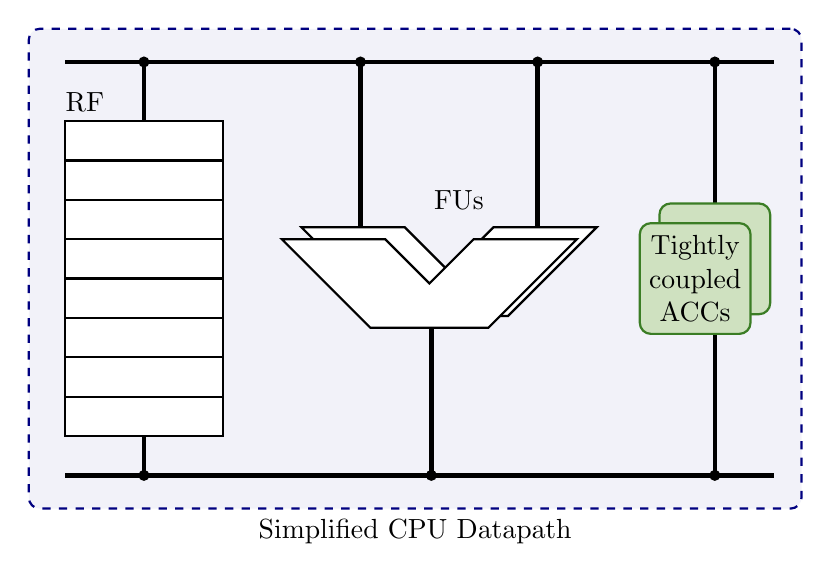
\begin{tikzpicture}
  \tikzstyle{coord}=[inner sep=0pt, outer sep=0pt, node distance=0pt]
  \tikzstyle{hwacc}=[rounded corners, draw=OliveGreen, fill=OliveGreen!20, thick, minimum size=40pt]
  \tikzstyle{control}=[draw=Purple, dashed, thick]
  \begin{scope}[name=datapath, local bounding box=dpathbb]

    % busses
    \draw[ultra thick] (0, 0.25) -- ++(9, 0);
    \draw[ultra thick] (0, -5) -- ++(9, 0);
    \draw[ultra thick] (1, 0.25) node [circle, minimum size=4pt, fill, inner sep=0pt] {} -- ++(0, -1);
    \draw[ultra thick] (3.75, 0.25) node [circle, minimum size=4pt, fill, inner sep=0pt] {} -- ++(0, -2.5);
    \draw[ultra thick] (6, 0.25) node [circle, minimum size=4pt, fill, inner sep=0pt] {} -- ++(0, -2.5);
    \draw[ultra thick] (8.25, 0.25) node [circle, minimum size=4pt, fill, inner sep=0pt] {} -- (8.25, -1.75);

    \draw[ultra thick] (1, -5) node [circle, minimum size=4pt, fill, inner sep=0pt] {} -- ++(0, 2);
    \draw[ultra thick] (4.65, -5) node [circle, minimum size=4pt, fill, inner sep=0pt] {} -- ++(0, 2.5);
    \draw[ultra thick] (8.25, -5) node [circle, minimum size=4pt, fill, inner sep=0pt] {} -- ++(0, 2.5);


    % register file drawing
    \begin{scope}[name=rf, local bounding box=rfbb, shift={(0, -0.5)}]
      \node at (0.25,0) [anchor=south] {RF};
      \draw[fill=white, thick] (0,0) rectangle (2, -4);
      \foreach \i in {1,...,8} {
        \node (rfout\i) at (2, -0.5*\i+0.25) [coord] {};
        \node (rfin\i) at (0, -0.5*\i+0.25) [coord] {};
        \draw[thick] (0, -0.5*\i) -- (2, -0.5*\i);
      }
    \end{scope}

    % functional units
    \begin{scope}[name=fu, local bounding box=fubb, shift={(6.5, -2)}]
      \node at (-1.5, 0.25) [anchor=south] {FUs};
      \begin{scope}[shift={(0.25, 0.15)}, rotate=-90, scale=0.75]
        \draw [fill=white, thick] (0, 0) -- (0, -1.75) -- (0.75, -2.5) -- (0, -3.25) -- (0, -5) -- (1.5, -3.5) -- (1.5, -1.5)
        -- cycle;
      \end{scope}
      \begin{scope}[rotate=-90, scale=0.75]
        \draw [fill=white, thick] (0, 0) -- node [coord] (alua) {} (0, -1.75) -- (0.75, -2.5) -- (0, -3.25)
        -- node [coord] (alub) {}
        (0, -5) -- (1.5, -3.5) -- node [coord] (alux) {} (1.5, -1.5) -- cycle;
      \end{scope}
    \end{scope}

    % tightly coupled accs
    \begin{scope}[shift={(8, -2.5)}]
      \node (hwacc2) at (0.25, 0.25) [hwacc] {};
      \node (hwacc1) at (0, 0) [hwacc, align=center] {Tightly\\coupled\\ ACCs};
    \end{scope}


  \end{scope}

  % \node (datamem) at (8.5, -2.5) [rounded corners, draw, thick, minimum size=50pt, align=center] {Data\\ Mem};
  % \node (instmem) at (8.5, -6) [rounded corners, draw, thick, minimum size=50pt, align=center] {Instr\\ Mem};

  \begin{scope}[on background layer]
    \node [fit=(dpathbb), draw=NavyBlue, fill=NavyBlue!5, rounded corners, dashed, thick, inner sep=10pt,
    label={270:Simplified CPU Datapath}] {};
  \end{scope}
\end{tikzpicture}
\end{document}